\documentclass[]{article}
\usepackage[left=1in,top=1in,right=1in,bottom=1in]{geometry}


%%%% more monte %%%%
  % thispagestyle{empty}
% https://stackoverflow.com/questions/2166557/how-to-hide-the-page-number-in-latex-on-first-page-of-a-chapter
\usepackage{color}
% \usepackage[table]{xcolor} % are they using color?
  
  % \definecolor{WSU.crimson}{HTML}{981e32}
% \definecolor{WSU.gray}{HTML}{5e6a71}

% \definecolor{shadecolor}{RGB}{248,248,248}
\definecolor{WSU.crimson}{RGB}{152,30,50} % use http://colors.mshaffer.com to convert from 981e32
\definecolor{WSU.gray}{RGB}{94,106,113}

%%%%%%%%%%%%%%%%%%%%%%%%%%%%
  
  \newcommand*{\authorfont}{\fontfamily{phv}\selectfont}
    \usepackage{lmodern}
  
  
  \usepackage[T1]{fontenc}
\usepackage[utf8]{inputenc}




\usepackage{abstract}
\renewcommand{\abstractname}{}    % clear the title
\renewcommand{\absnamepos}{empty} % originally center

\renewenvironment{abstract}
{{%
  \setlength{\leftmargin}{0mm}
  \setlength{\rightmargin}{\leftmargin}%
}%
  \relax}
{\endlist}

\makeatletter
\def\@maketitle{%
  \pagestyle{empty}
  \newpage
  %  \null
  %  \vskip 2em%
    %  \begin{center}%
    \let \footnote \thanks
  {\fontsize{18}{20}\selectfont\raggedright  \setlength{\parindent}{0pt} \@title \par}%
}
%\fi
\makeatother


  
  
  
  
        \usepackage{color}
  \usepackage{fancyvrb}
  \newcommand{\VerbBar}{|}
  \newcommand{\VERB}{\Verb[commandchars=\\\{\}]}
  \DefineVerbatimEnvironment{Highlighting}{Verbatim}{commandchars=\\\{\}}
  % Add ',fontsize=\small' for more characters per line
  \usepackage{framed}
  \definecolor{shadecolor}{RGB}{248,248,248}
  \newenvironment{Shaded}{\begin{snugshade}}{\end{snugshade}}
  \newcommand{\AlertTok}[1]{\textcolor[rgb]{0.94,0.16,0.16}{#1}}
  \newcommand{\AnnotationTok}[1]{\textcolor[rgb]{0.56,0.35,0.01}{\textbf{\textit{#1}}}}
  \newcommand{\AttributeTok}[1]{\textcolor[rgb]{0.77,0.63,0.00}{#1}}
  \newcommand{\BaseNTok}[1]{\textcolor[rgb]{0.00,0.00,0.81}{#1}}
  \newcommand{\BuiltInTok}[1]{#1}
  \newcommand{\CharTok}[1]{\textcolor[rgb]{0.31,0.60,0.02}{#1}}
  \newcommand{\CommentTok}[1]{\textcolor[rgb]{0.56,0.35,0.01}{\textit{#1}}}
  \newcommand{\CommentVarTok}[1]{\textcolor[rgb]{0.56,0.35,0.01}{\textbf{\textit{#1}}}}
  \newcommand{\ConstantTok}[1]{\textcolor[rgb]{0.00,0.00,0.00}{#1}}
  \newcommand{\ControlFlowTok}[1]{\textcolor[rgb]{0.13,0.29,0.53}{\textbf{#1}}}
  \newcommand{\DataTypeTok}[1]{\textcolor[rgb]{0.13,0.29,0.53}{#1}}
  \newcommand{\DecValTok}[1]{\textcolor[rgb]{0.00,0.00,0.81}{#1}}
  \newcommand{\DocumentationTok}[1]{\textcolor[rgb]{0.56,0.35,0.01}{\textbf{\textit{#1}}}}
  \newcommand{\ErrorTok}[1]{\textcolor[rgb]{0.64,0.00,0.00}{\textbf{#1}}}
  \newcommand{\ExtensionTok}[1]{#1}
  \newcommand{\FloatTok}[1]{\textcolor[rgb]{0.00,0.00,0.81}{#1}}
  \newcommand{\FunctionTok}[1]{\textcolor[rgb]{0.00,0.00,0.00}{#1}}
  \newcommand{\ImportTok}[1]{#1}
  \newcommand{\InformationTok}[1]{\textcolor[rgb]{0.56,0.35,0.01}{\textbf{\textit{#1}}}}
  \newcommand{\KeywordTok}[1]{\textcolor[rgb]{0.13,0.29,0.53}{\textbf{#1}}}
  \newcommand{\NormalTok}[1]{#1}
  \newcommand{\OperatorTok}[1]{\textcolor[rgb]{0.81,0.36,0.00}{\textbf{#1}}}
  \newcommand{\OtherTok}[1]{\textcolor[rgb]{0.56,0.35,0.01}{#1}}
  \newcommand{\PreprocessorTok}[1]{\textcolor[rgb]{0.56,0.35,0.01}{\textit{#1}}}
  \newcommand{\RegionMarkerTok}[1]{#1}
  \newcommand{\SpecialCharTok}[1]{\textcolor[rgb]{0.00,0.00,0.00}{#1}}
  \newcommand{\SpecialStringTok}[1]{\textcolor[rgb]{0.31,0.60,0.02}{#1}}
  \newcommand{\StringTok}[1]{\textcolor[rgb]{0.31,0.60,0.02}{#1}}
  \newcommand{\VariableTok}[1]{\textcolor[rgb]{0.00,0.00,0.00}{#1}}
  \newcommand{\VerbatimStringTok}[1]{\textcolor[rgb]{0.31,0.60,0.02}{#1}}
  \newcommand{\WarningTok}[1]{\textcolor[rgb]{0.56,0.35,0.01}{\textbf{\textit{#1}}}}
        
    
  
    \title{\textbf{\textcolor{WSU.crimson}{The 8 Stacked Heads Test}} \newline \textbf{\textcolor{WSU.gray}{STAT 419: Project Measure}}  }
  
  %  
  
  % \author{ \Large true \hfill \normalsize \emph{} }
\author{\Large Kathleen Rivas\vspace{0.05in} \newline\normalsize\emph{Washington State University}  }
  
  
  \date{November 10, 2020}
\setcounter{secnumdepth}{3}

\usepackage{titlesec}
% See the link above: KOMA classes are not compatible with titlesec any more. Sorry.
% https://github.com/jbezos/titlesec/issues/11
\titleformat*{\section}{\bfseries}
\titleformat*{\subsection}{\bfseries\itshape}
\titleformat*{\subsubsection}{\itshape}
\titleformat*{\paragraph}{\itshape}
\titleformat*{\subparagraph}{\itshape}

% https://code.usgs.gov/usgs/norock/irvine_k/ip-092225/
  
  
  %\titleformat*{\section}{\normalsize\bfseries}
%\titleformat*{\subsection}{\normalsize\itshape}
%\titleformat*{\subsubsection}{\normalsize\itshape}
%\titleformat*{\paragraph}{\normalsize\itshape}
%\titleformat*{\subparagraph}{\normalsize\itshape}

% https://tex.stackexchange.com/questions/233866/one-column-multicol-environment#233904
\usepackage{environ}
\NewEnviron{auxmulticols}[1]{%
  \ifnum#1<2\relax% Fewer than 2 columns
  %\vspace{-\baselineskip}% Possible vertical correction
  \BODY
  \else% More than 1 column
  \begin{multicols}{#1}
    \BODY
    \end{multicols}%
    \fi
  }
  
  
  
  
  
      \usepackage{natbib}
  \setcitestyle{aysep={}} %% no year, comma just year
  % \usepackage[numbers]{natbib}
  \bibliographystyle{./../biblio/ormsv080.bst}
  
  
  
  \usepackage[strings]{underscore} % protect underscores in most circumstances
      
    
        
    
    \newtheorem{hypothesis}{Hypothesis}
  \usepackage{setspace}
  
  
  %%%%%%%%%%%%%%%%%%%%%%%%%%%%%%%%%%%%%%%%%%%%%%%%%%%%%
  %%% MONTE ADDS %%%
    
    \usepackage{fancyhdr} % fancy header 
  \usepackage{lastpage} % last page 
  
  \usepackage{multicol}
  
  
  \usepackage{etoolbox}
  \AtBeginEnvironment{quote}{\singlespacing\small}
  % https://tex.stackexchange.com/questions/325695/how-to-style-blockquote
  
  
  \usepackage{soul}			%% allows strike-through
  \usepackage{url}			%% fixes underscores in urls
  \usepackage{csquotes}		%% allows \textquote in references
  \usepackage{rotating}		%% allows table and box rotation
  \usepackage{caption}		%% customize caption information
  \usepackage{booktabs}		%% enhance table/tabular environment
  \usepackage{tabularx}		%% width attributes updates tabular
  \usepackage{enumerate}		%% special item environment
  \usepackage{enumitem}		%% special item environment
  
  \usepackage{lineno}		%% allows linenumbers for editing using \linenumbers
  \usepackage{hanging}
  
  
  \usepackage{mathtools}  	%% also loads amsmath
  \usepackage{bm}		%% bold-math
  \usepackage{scalerel}	%% scale one element (make one beta bigger font)
  
  \newcommand{\gFrac}[2]{ \genfrac{}{}{0pt}{1}{{#1}}{#2} }
    
    \newcommand{\betaSH}[3]{  \gFrac{\text{\tiny #1}}{{\text{\tiny #2}}}\hat{\beta}_{\text{#3}}   }
      \newcommand{\betaSB}[3]{              ^{\text{#1}} _{\text{#2}} \bm{\beta} _{\text{#3}}                   }  %% bold
        \newcommand{\bigEQ}{  \scaleobj{1.5}{{\ }= } }
        \newcommand{\bigP}[1]{  \scaleobj{1.5}{#1 } }
          
          
          
          
          
          \usepackage{endnotes}  % he already does this ...
          \renewcommand{\enotesize}{\normalsize}
          % https://tex.stackexchange.com/questions/99984/endnotes-do-not-be-superscript-and-add-a-space
          \renewcommand\makeenmark{\textsuperscript{[\theenmark]}} % in brackets %
            % https://tex.stackexchange.com/questions/31574/how-to-control-the-indent-in-endnotes
          \patchcmd{\enoteformat}{1.8em}{0pt}{}{}
          
          \patchcmd{\theendnotes}
          {\makeatletter}
          {\makeatletter\renewcommand\makeenmark{\textbf{[\theenmark]} }}
          {}{}
          
          
          
          % https://tex.stackexchange.com/questions/141906/configuring-footnote-position-and-spacing
          
          \addtolength{\footnotesep}{5mm} % change to 1mm
          
          \renewcommand{\thefootnote}{\textbf{\arabic{footnote}}}
          \let\footnote=\endnote
          %\renewcommand*{\theendnote}{\alph{endnote}}
          %\renewcommand{\theendnote}{\textbf{\arabic{endnote}}}
          
          
          \renewcommand*{\notesname}{ENDNOTES}
          
          \makeatletter
          \def\enoteheading{\section*{\notesname
            \@mkboth{\MakeUppercase{\notesname}}{\MakeUppercase{\notesname}}}%
            \mbox{}\par\vskip-2.3\baselineskip\noindent\rule{.5\textwidth}{0.4pt}\par\vskip\baselineskip}
          \makeatother
          
          
          \renewcommand*{\contentsname}{TABLE OF CONTENTS}
          
          \renewcommand*{\refname}{REFERENCES}
          
          
          %\usepackage{subfigure}
          \usepackage{subcaption}
          
          \captionsetup{labelfont=bf}  % Make Table / Figure bold
          
          %%% you could add elements here ... monte says .... %%%
            %\usepackage{mypackageForCapitalH}
          
          
          %%%%%%%%%%%%%%%%%%%%%%%%%%%%%%%%%%%%%%%%%%%%%%%%%%%%%
          
          % set default figure placement to htbp
          \makeatletter
          \def\fps@figure{htbp}
          \makeatother
          
                      
            % move the hyperref stuff down here, after header-includes, to allow for - \usepackage{hyperref}
          
          \makeatletter
          \@ifpackageloaded{hyperref}{}{%
            \ifxetex
            \PassOptionsToPackage{hyphens}{url}\usepackage[setpagesize=false, % page size defined by xetex
                                                           unicode=false, % unicode breaks when used with xetex
                                                           xetex]{hyperref}
            \else
              \PassOptionsToPackage{hyphens}{url}\usepackage[draft,unicode=true]{hyperref}
            \fi
          }
          
          \@ifpackageloaded{color}{
            \PassOptionsToPackage{usenames,dvipsnames}{color}
          }{%
            \usepackage[usenames,dvipsnames]{color}
          }
          \makeatother
          \hypersetup{breaklinks=true,
          bookmarks=true,
          pdfauthor={Kathleen Rivas (Washington State University)},
          pdfkeywords = {summary statistics; correlation; korean beauty standards},  
          pdftitle={The 8 Stacked Heads Test: STAT 419: Project Measure},
          colorlinks=true,
          citecolor=blue,
          urlcolor=blue,
          linkcolor=magenta,
          pdfborder={0 0 0}}
          \urlstyle{same}  % don't use monospace font for urls

% Add an option for endnotes. -----

%
% add tightlist ----------
\providecommand{\tightlist}{%
\setlength{\itemsep}{0pt}\setlength{\parskip}{0pt}}

% add some other packages ----------

% \usepackage{multicol}
% This should regulate where figures float
% See: https://tex.stackexchange.com/questions/2275/keeping-tables-figures-close-to-where-they-are-mentioned
\usepackage[section]{placeins}



\pagestyle{fancy}   
\lhead{\textcolor{WSU.crimson}{\textbf{ The 8 Stacked Heads Test }}}
\chead{}
\rhead{\textcolor{WSU.gray}{\textbf{  Page\ \thepage\ of\ \protect\pageref{LastPage} }}}
\lfoot{}
\cfoot{}
\rfoot{}


\begin{document}
	
% \pagenumbering{arabic}% resets `page` counter to 1 
%
% \maketitle

{% \usefont{T1}{pnc}{m}{n}
\setlength{\parindent}{0pt}
\thispagestyle{plain}
{\fontsize{18}{20}\selectfont\raggedright 
\maketitle  % title \par  

}

{
   \vskip 13.5pt\relax \normalsize\fontsize{11}{12} 
   
\textbf{\authorfont Kathleen Rivas} \hskip 15pt \emph{\small Washington State University}   

}

}








\begin{abstract}

    \hbox{\vrule height .2pt width 39.14pc}

    \vskip 8.5pt % \small 

\noindent In this article I compare the head to height proportion from a dataset
gathered by students in a large public university statistics class. I
look at correlation of head to height proportion and gender, and head to
height and ethnicity.


\vskip 8.5pt \noindent \textbf{\underline{Keywords}:} summary statistics; correlation; korean beauty standards \par

    




    
    \hbox{\vrule height .2pt width 39.14pc}
    \vskip 5pt 
    \hfill \textbf{\textcolor{WSU.gray}{ November 10, 2020 } }
    \vskip 5pt 
    
\end{abstract}


\vskip -8.5pt



 % removetitleabstract

\noindent  

\section{Introduction}
\label{sec:intro}

The saying goes, \enquote{Beauty is in the eye of the beholder.}
However, in Korean culture, this is a very specific image, for both
genders. Korea is considered the \enquote{world's plastic surgery
capital.} \citep{Jacobs:2018} One of the more unusual beauty standard in
Korea is to have a \enquote{small head.} It is called the \enquote{8
Stacked heads} test. If the height is the length of 8 \enquote{heads}
(the length of your head from the top of the head to the bottom of the
chin), then you are considered attractive. This standard applies to all
genders. \citep{Koreaboo:2017}

{[}ONE GRAPHIC -- I am breaking report form to state that I did not have
time to make a graphic. But if I did, I would construct it similar to
the weather graphic you created. The bottom row would have the range of
head to height proportions, and across the graphic would be the data
points. Different color/shape to denote gender. Different colors below
it to denote ethnicity points.{]}

\section{Research Question:  How realistic is the "8 Stacked Heads" test?}
\label{sec:rq}

Beauty standards are often unrealistic, but I was curious to see how
realistic this particular beauty standard was. I have heard about
Koreans preference for \enquote{small heads}, and anecdotally, have come
across several Caucasian male and Asian female partners where the taller
Caucasian male would often have head circumference sizes smaller than
their Asian female partners. These personal experiences have caused me
to wonder if Asians have larger heads in proportion to their height, in
general, causing this peculiar beauty standard of having a
\enquote{small head.} Getting a sample size greater than I could collect
on my own gives me the opportunity to explore this beauty standard in
greater detail than a handful of anecdotal experiences.

\subsection{Is there a correlation between the likelihood of meeting this beauty standard and ethnicity or gender?}
\label{sec:rq2}

The overall question is rather simple, and can be found by getting the
mean of the stacked heads ratio. What is more interesting is to see if
there is any correlation between ethnicity, gender, and the stacked
heads ratio.

\section{Data Description}
\label{sec:data}

Method

Participants and procedure: Students enrolled in data analytics
statistics class at a large state university participated as well as
gathered different bodily measurements. The sample(N=428, 72.2\%
Caucasian), with a median age of 34.4. Measures were gathered from a
variety of methods, from online, to the student personally gathering
measurements on a participant. The participants were connected by
personal network of students in the statistics class.

Measures: Items gathered were of different body measurements. Most of
them were gathered horizontally or vertically, but head circumference
was also gathered. Covariates such as eye color and dominant hand for
writing and swinging were included. The full measures are shown in the
Appendix.

To gather evidence for the correlation and summary statistics for the
Korean head to height beauty ideal of 7 to 8 \enquote{heads} from the
neck down, measurements of height and the length of head from top of the
head to below the chin. Other measures gathered for this study was
ethnicity, gender, and age.

After data cleansing, the sample used for analysis reduced to N=231. The
quality was determined on the scale of 1-10.

\subsection{Summary of Sample}
\label{sec:data-sample}

The sample (N=231) covariates consisted of 118 males, 112 females, 1
other. The age ranged from 3 to 94 years.\\
\vspace{5mm}

\begin{tabular}{ c c c c c}
  Caucasian & Asian & Hispanic & African-American & Other \\
  \hline
  167 & 39 & 7 & 8 & 10
\end{tabular}
\vspace{5mm}

\begin{tabular}{ c c c c c}
   Caucasian & Asian & Hispanic & African-American & Other \\
  \hline
  72.2\% & 16.9\% & 3\% & 3.5\% & 4.3\%
\end{tabular}

\subsection{Summary Statistics of Data}
\label{sec:data-summary}

According to the correlation table, there is no strong correlation
between \enquote{passing} the \enquote{8 Stacked Heads} test and any
factor (such as ethnicity or gender). There is a weak correlation
between ethnicity and head to height proportion (p = -.16). Here is the
breakdown of those that \enquote{passed} the test: \vspace{5mm}

\begin{tabular} {c c}
  Male & Female \\ 
  \hline
  34.745\% & 34.821\%
\end{tabular}
\vspace{5mm}

\begin{tabular} { c c c c c}
  Caucasian & Asian & Hispanic & African-American & Other \\
  \hline
  38\% & 18\% & 14\% & 62.5\% & 30\%
\end {tabular}

\section{Key Findings}
\label{sec:findings}

80 out of 231 participants met the \enquote{8 Stacked Heads} beauty
standard (34.632\%). As expected, this is not a common measurement
people \enquote{attain}. The largest ethnicity group was Caucasian, and
the population that \enquote{passed} the test roughly matches the
proportion of all ethnicities that passed the test -- Caucasian 38\% and
total 34.632\%. The second largest group is Asian, with 39 participants
in this category -- not a large dataset to work with, but interestingly,
only 18\% passed this test, significantly lower than 34.632\%. Also
interesting, is the percentage of African-American which is
significantly higher at 62.5\% vs 34.632\%. \enquote{Other} comprises of
Indian, Native Americans, and mixed heritage, and fall in at 30\% --
close to the total. The Hispanic group is also low, lower than Asian at
14\%, but I looked at the dataset manually (because it was so small at
only 8 participants), and some of the proportions seem unusually small
as to make me question the quality of the data. For example, a 26 year
old Asian with a ratio of 4.4667 heads. I mean\ldots it's
possible\ldots but I question it?

I have noticed (but not been able to statistically derive) that age can
play a factor -- children's head to height proportions seem to be lower
(i.e.~children's heads are larger in proportion to their bodies) on
average.

\section{Conclusion}
\label{sec:conclusion}

Overall, the dataset proves to me that Asians have a lower
\enquote{chance} of \enquote{passing} the \enquote{8 Stacked Heads} test
which might be why, as a society, they have having a \enquote{small
head} as determined by the \enquote{8 Stacked Heads} test. Not that I've
talked to an exhaustive amount of non-Asians, but again, anecdotally,
non-Asians do not share this Korean beauty standard and mystified and
confused as to how this could be considered a beauty standard. If the
average, as well as Caucasians pass this \enquote{test} at 34.632 -
38\%, and Asians pass at 18\%, this would be a soft \enquote{proof} my
suspicions that Asians have \enquote{big} heads, in general, therefore
they view \enquote{small} heads as rare, and therefore more beautiful.

\newpage

\begin{figure}[!ht]
%% figures have hrule, tables have hline
    \hrule
    \caption{ \textbf{Korean-Talk-Show-Where-Celebrities-Get-Tested} }
    \begin{center}
        \scalebox{1.00}{    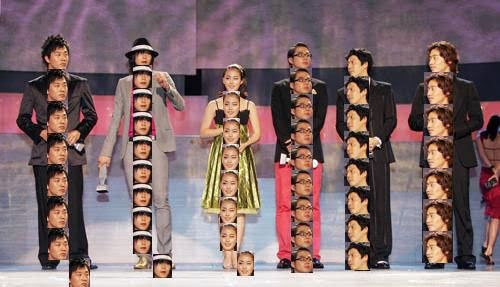
\includegraphics[trim = 0 0 0 0,clip,width=\textwidth]{figures/Koreaboo.jpg} }
    \end{center}
    \label{fig:Koreaboo-Image}
    \hrule
\end{figure}

\newpage

\begin{table}[!htbp]
\footnotesize
\centering
\caption{\textbf{Descriptive Statistics and Correlation Analysis}}
\label{table:correlation}
\begin{tabularx}{0.95\textwidth}{{r@{ \ \ } p{35mm} r@{}lp{1mm} r@{}l p{5mm} r@{}l p{2mm} r@{}l p{2mm} r@{}l p{2mm}   r@{}l  }}
 & \\
\hline
 & \\
\multicolumn{2}{c}{\textbf{ }} & \multicolumn{2}{c}{\textbf{M}} & & \multicolumn{2}{c}{\textbf{SD}} &  & \multicolumn{2}{c}{\textbf{1}} &  & \multicolumn{2}{c}{\textbf{2}} &  & \multicolumn{2}{c}{\textbf{3}} &  & \\ 
 & \\
\hline
 & \\
\textbf{1} & \textbf{Head to Height} &  6&.7 &  &  &.87 &  &  1&  &  &  \multicolumn{2}{c}{ \  \  \  \  \ }  &  &  \multicolumn{2}{c}{ \  \  \  \  \ }  &  & \\ 
 & \\
\textbf{2} & \textbf{Ethnicity} &  1&.5 &  &  1&.02 &  &  -&.16{$^{*}$}  &  &  1&  &  &  \multicolumn{2}{c}{ \  \  \  \  \ }  &  & \\ 
 & \\
\textbf{3} & \textbf{Age} &  34&.4 &  &  17&.68 &  &  -&.02 &  &  -&.12{$^{\dagger}$}  &  &  1&  &  & \\ 
 & \\
\textbf{4} & \textbf{Gender} &  1&.5 &  &  &.51 &  &  &.07 &  &  -&.01 &  &  -&.08 &  & \\ 
 & \\
\hline
 & \\
\multicolumn{16}{p{0.86\textwidth}}{  \footnotesize { \begin{hangparas}{0.75in}{1} \textbf{\underline{Notes}:} \ \ Pearson pairwise correlations are reported; \newline a two-side test was performed to report correlation significance.  \end{hangparas} } }  & \\  
\multicolumn{16}{p{0.86\textwidth}}{  {\tiny {$^{\dagger} p < .10$} }  {     } {\tiny        {$^{*} p < .05$} }  {     } {\tiny       {$^{**} p < .01$} }  {     } {\tiny      {$^{***} p < .001$} } {     }     } & \\ 
 & \\
\hline
\end{tabularx}
\end{table}


\newpage

\section{APPENDICES}
\label{sec:appendix}

\subsection{Data Provenance}
\label{sec:appendix-data-provenance}

Data Provenance was implemented with the usage of Github for version
control, and the original dataset was not modified. Analysis was done on
separate, reproducible copies. Data collection was less rigorous, as I
did not have direct control over all measurements gathering, but data
cleansing was done to remove NAs, duplicates, and data that did not look
genuine.

The data was collected by a WSU statistics class, and was tasked to find
measure a total of 10 people for the various following measurements and
covariates:\vspace{5mm}

Height: standing height, preferably with no shoes on

Head Height: height from the top of the head to below the chin

Head Circumference: distance around head, measured right above ears or
eyes

Hand Length: length of hand from middle finger to wrist

Hand Width: width of hand from pinkie finger to thumb fully stretched

Hand to Elbow: length from middle finger to elbow

Elbow to Armpit: length from elbow to armpit

Arm Reach: standing flat footed, length from floor to the extended arm
maximum point

Arm Span: length from each middle finger, fully extended

Foot Length: length of foot from largest toe to back of heel

Floor to Kneepit: distance from floor to the kneepit

Floor to Hip: distance from the floor to the hip (top of the pantline)

Floor to Navel: distance from the floor to the navel, orthogonal
measurement

Floor to Armpit: distance from floor to the armpit \vspace{5mm}

Covariates:

Measurement unit: centimeters, inches

Dominant writing hand: left, right, both

Eye Color: brown, green, blue, hazel

Dominant swinging arm/hand: left, right, both

Age

Gender: male, female, other

Quality of measurements: 1-10

Minutes: length of minutes

Ethnicity

Miscellaneous notes on the subject and the data collection \vspace{5mm}

Part of responsible data collection is the need for the data to be both
quality and anonymous to protect the subjects. Data privacy was a huge
component discussed in my Data Ethics class -- and for this project,
students were asked to anonymize names to protect privacy. This project
also does not make the original dataset publicly available as well to
protect identities.

\newpage
\subsubsection{Data Collection Handout}
\label{sec:appendix-data-handout}

\begin{figure}[!ht]
    \hrule
    \caption{ \textbf{Handout} }
    \begin{center}
        \scalebox{1.00}{    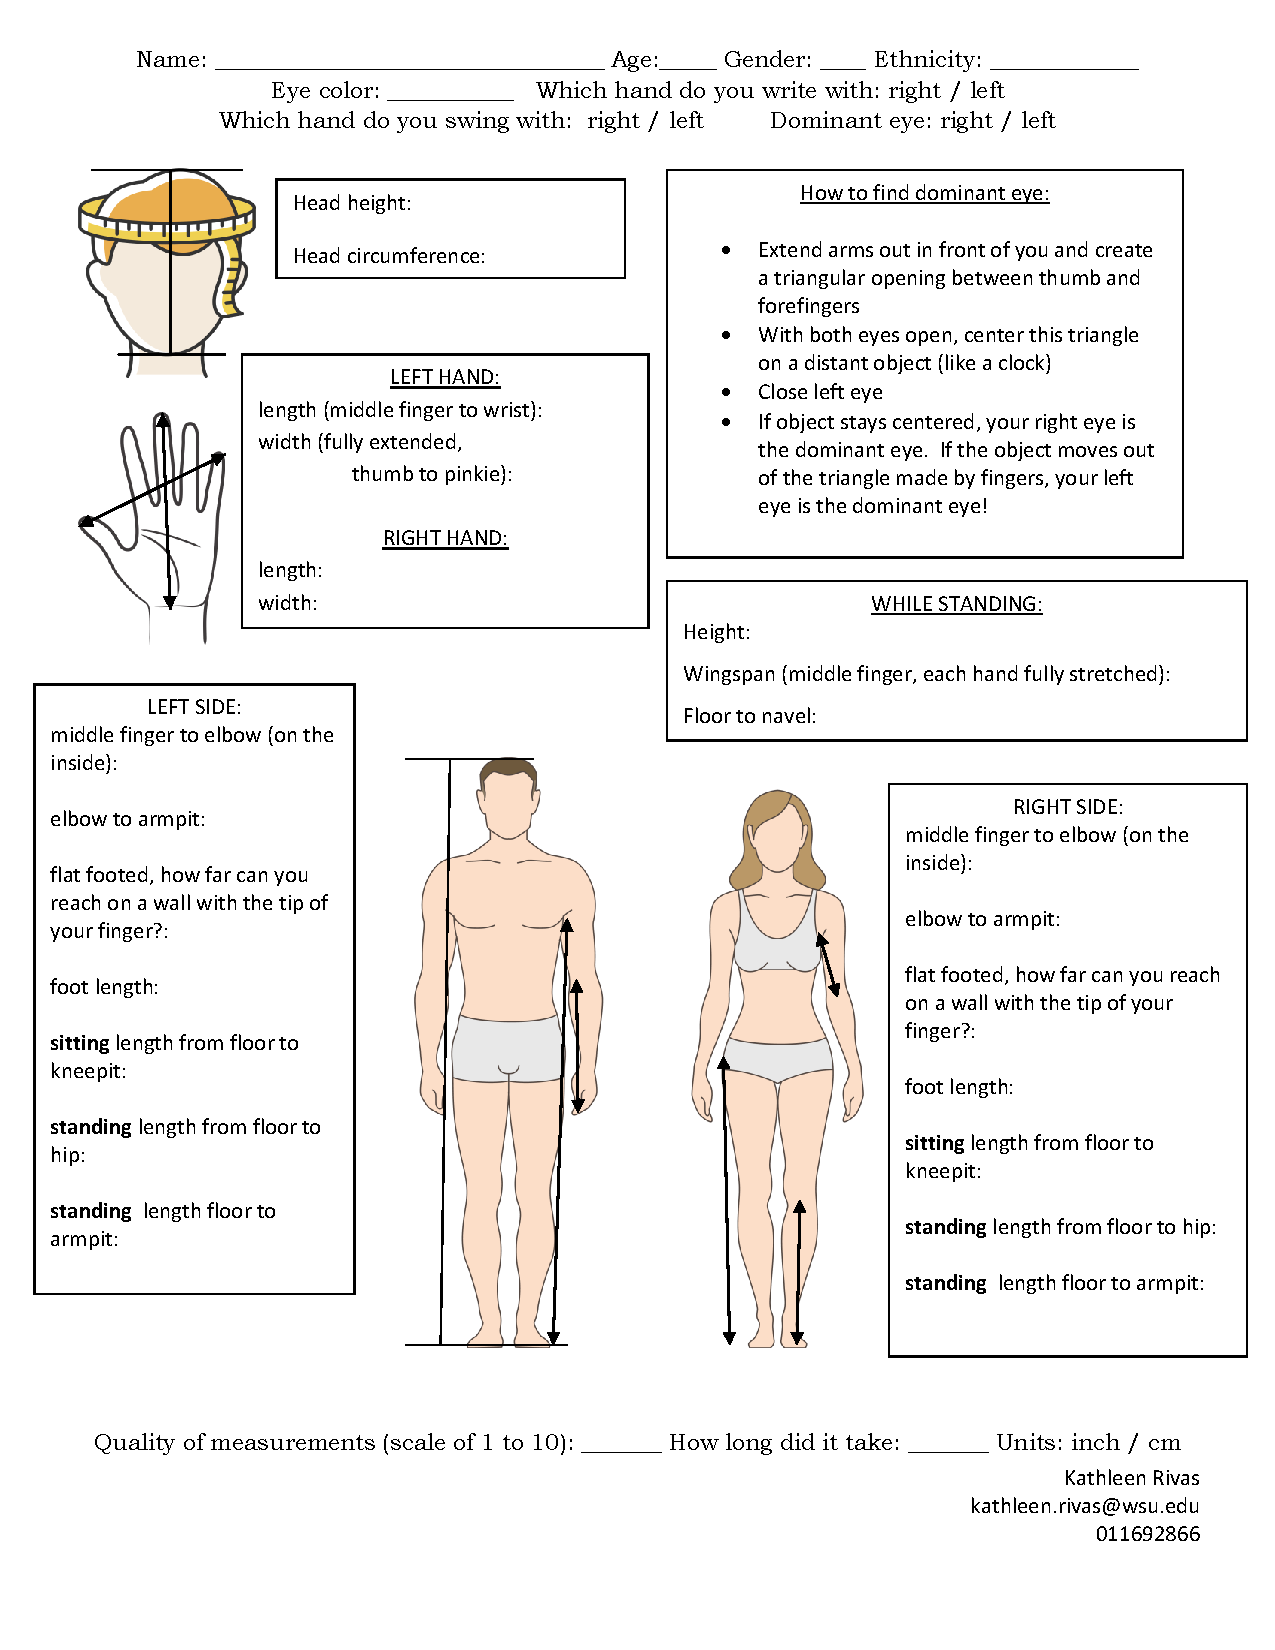
\includegraphics[trim = 0 0 0 0,clip,width=0.85\textwidth]{pdfs/project_01_handout.pdf} }
    \end{center}
    \label{fig:handout-1}
    \hrule
\end{figure}

\newpage

\subsection{Personal Opinion}
\label{sec:appendix-personl-opinion}

I feel that some Asian beauty standards are an attempt to look more
\enquote{Westernized}, however, most are not. Most are traditionally
rooted in their ideas of beauty for centuries -- such as their obsession
with white skin, small head, and thinness. Non-Asian females are
pressured to be thin to be beautiful, but not to the degree Asian
females are. On the other hand, breast nor butt size matters not in
Asian culture for the most part, comparatively to Western culture.\\
\vspace{5mm} It is too bad that I have not had more time (not implying
you should have extended this deadline further, it's more an implication
of my personal lack of time between other classes and personal life) or
a larger dataset to work with. Also, I should have thought about the
type of measurements gathered first before I settled on a research
question. I wanted to flesh out the project with several beauty
standards, namely revolving around waist to hip (WTR) or waist to
shoulder (for male standard), but when I finally got to analysis, I
realized that I didn't have waist measurements. That's a lesson for me
-- to look at the dataset to see if I am able to answer my question with
it or does the dataset not support the query.

\newpage

\subsection{Preparing the Report Workspace as a subsection}
\label{sec:appendix-setup}

\subsubsection{Preparing the Report Workspace as a subsubsection}
\label{sec:appendix-setup2}

\paragraph{Preparing the Report Workspace as a paragraph}
\label{sec:appendix-setup3}

\subparagraph{Preparing the Report Workspace as a subparagrah}
\label{sec:appendix-setup4}

Below is the necessary functions and libraries required to run the code
referenced in this document.

\begin{Shaded}
\begin{Highlighting}[]
\KeywordTok{library}\NormalTok{(devtools);       }\CommentTok{# required for source_url}
\KeywordTok{library}\NormalTok{(dplyr)}

\NormalTok{path.humanVerseWSU =}\StringTok{ "https://raw.githubusercontent.com/MonteShaffer/humanVerseWSU/"}
\KeywordTok{source_url}\NormalTok{( }\KeywordTok{paste0}\NormalTok{(path.humanVerseWSU,}\StringTok{"master/misc/functions-project-measure.R"}\NormalTok{) );}
\end{Highlighting}
\end{Shaded}

\begin{verbatim}
## Warning: package 'Hmisc' was built under R version 4.0.3
\end{verbatim}

Below is the code to load the data and prepare it for analysis.

\begin{Shaded}
\begin{Highlighting}[]
\NormalTok{path.project =}\StringTok{ "C:/_git_/WSU_STATS419_FALL2020/project-measure/"}\NormalTok{;}

\NormalTok{path.github =}\StringTok{ "https://raw.githubusercontent.com/kat-rivas/WSU_STATS419_FALL2020/"}\NormalTok{;}
\KeywordTok{source_url}\NormalTok{( }\KeywordTok{paste0}\NormalTok{(path.github,}\StringTok{"master/functions/functions-project-measure.R"}\NormalTok{) );}

\NormalTok{measure =}\StringTok{ }\KeywordTok{readRDS}\NormalTok{(}\StringTok{"C:/Users/Dorbs of Doom/Documents/WSU/Fall 2020/STAT 419 Intro to Multivariate/final.measure.rds"}\NormalTok{)}

\NormalTok{measure.df =}\StringTok{ }\KeywordTok{prepareMeasureData}\NormalTok{(measure)}
\end{Highlighting}
\end{Shaded}

Below is the code to generate the summary statistics and save them as a
table that you see in Section \ref{}.

\begin{Shaded}
\begin{Highlighting}[]
\KeywordTok{library}\NormalTok{(devtools);       }\CommentTok{# required for source_url}
\KeywordTok{library}\NormalTok{(dplyr)}

\NormalTok{path.humanVerseWSU =}\StringTok{ "https://raw.githubusercontent.com/MonteShaffer/humanVerseWSU/"}
\KeywordTok{source_url}\NormalTok{( }\KeywordTok{paste0}\NormalTok{(path.humanVerseWSU,}\StringTok{"master/misc/functions-project-measure.R"}\NormalTok{) );}

\NormalTok{path.project =}\StringTok{ "C:/Users/Dorbs of Doom/_git_/WSU_STATS419_FALL2020/project-measure/"}\NormalTok{;}
\NormalTok{path.tables =}\StringTok{ }\KeywordTok{paste0}\NormalTok{(path.project,}\StringTok{"tables/"}\NormalTok{);}
  \KeywordTok{createDirRecursive}\NormalTok{(path.tables);}
\end{Highlighting}
\end{Shaded}

\begin{Shaded}
\begin{Highlighting}[]
\NormalTok{file.correlation =}\StringTok{ }\KeywordTok{paste0}\NormalTok{(path.tables,}\StringTok{"my-correlation-table.tex"}\NormalTok{);}

\NormalTok{measure.df =}\StringTok{ }\KeywordTok{prepareMeasureData}\NormalTok{(measure)}

\NormalTok{measure.df2 =}\StringTok{ }\KeywordTok{select}\NormalTok{(measure.df, head.to.height, ethnicity.groups, age, my.gender)}
\NormalTok{myData =}\StringTok{ }\KeywordTok{as.matrix}\NormalTok{(measure.df2);  }\CommentTok{# numeric values only, only what will appear in table}

\KeywordTok{buildLatexCorrelationTable}\NormalTok{(myData, }
  \DataTypeTok{rotateTable =} \OtherTok{FALSE}\NormalTok{,}
  \DataTypeTok{width.table =} \FloatTok{0.95}\NormalTok{, }\CommentTok{# best for given data ... 0.95 when rotateTable = FALSE}
                      \CommentTok{# 0.60 when rotateTable = TRUE}
  \DataTypeTok{myFile =}\NormalTok{ file.correlation,}
  \DataTypeTok{myNames =} \KeywordTok{c}\NormalTok{(}\StringTok{"Head to Height"}\NormalTok{,}\StringTok{"Ethnicity"}\NormalTok{, }\StringTok{"Age"}\NormalTok{, }\StringTok{"Gender"}\NormalTok{ ) );}


\KeywordTok{Sys.sleep}\NormalTok{(}\DecValTok{2}\NormalTok{); }\CommentTok{# in case Knit-PDF doesn't like that I just created the file...}
\end{Highlighting}
\end{Shaded}

\begin{Shaded}
\begin{Highlighting}[]
\NormalTok{total =}\StringTok{ }\KeywordTok{nrow}\NormalTok{(measure.df); total}
\end{Highlighting}
\end{Shaded}

\begin{verbatim}
## [1] 231
\end{verbatim}

\begin{Shaded}
\begin{Highlighting}[]
\NormalTok{ethnicity.freq =}\StringTok{ }\KeywordTok{table}\NormalTok{(measure.df2}\OperatorTok{$}\NormalTok{ethnicity.groups)}
\NormalTok{gender.freq =}\StringTok{ }\KeywordTok{table}\NormalTok{(measure.df2}\OperatorTok{$}\NormalTok{my.gender)}
\KeywordTok{mean}\NormalTok{(measure.df2}\OperatorTok{$}\NormalTok{head.to.height)}
\end{Highlighting}
\end{Shaded}

\begin{verbatim}
## [1] 6.656682
\end{verbatim}

\begin{Shaded}
\begin{Highlighting}[]
\CommentTok{#to find out how many meet the 8 stacked head}
\NormalTok{pass =}\StringTok{ }\DecValTok{0}
\KeywordTok{rownames}\NormalTok{(measure.df2) <-}\StringTok{ }\KeywordTok{seq}\NormalTok{(}\DataTypeTok{length=}\DecValTok{231}\NormalTok{)}
  
\ControlFlowTok{for}\NormalTok{ (i }\ControlFlowTok{in} \DecValTok{1}\OperatorTok{:}\KeywordTok{nrow}\NormalTok{(measure.df2))}
\NormalTok{\{}
  \ControlFlowTok{if}\NormalTok{ (measure.df2}\OperatorTok{$}\NormalTok{head.to.height[i] }\OperatorTok{>=}\StringTok{ }\DecValTok{7}\NormalTok{)}
\NormalTok{  \{}
\NormalTok{    pass =}\StringTok{ }\NormalTok{pass }\OperatorTok{+}\StringTok{ }\DecValTok{1}
\NormalTok{  \}}
  \ControlFlowTok{else}
\NormalTok{  \{}
    \ControlFlowTok{next}
\NormalTok{  \}}
\NormalTok{\}}
\NormalTok{pass}
\end{Highlighting}
\end{Shaded}

\begin{verbatim}
## [1] 80
\end{verbatim}

\begin{Shaded}
\begin{Highlighting}[]
\CommentTok{#to find out gender and head to height}
\NormalTok{male =}\StringTok{ }\DecValTok{0}
\NormalTok{female =}\StringTok{ }\DecValTok{0}
\ControlFlowTok{for}\NormalTok{ (i }\ControlFlowTok{in} \DecValTok{1}\OperatorTok{:}\DecValTok{231}\NormalTok{)}
\NormalTok{\{}
  \ControlFlowTok{if}\NormalTok{ (measure.df2[i,}\DecValTok{1}\NormalTok{] }\OperatorTok{>=}\StringTok{ }\DecValTok{7}\NormalTok{)}
\NormalTok{  \{}
    \ControlFlowTok{if}\NormalTok{ (measure.df2[i,}\DecValTok{4}\NormalTok{] }\OperatorTok{==}\StringTok{ "2"}\NormalTok{)}
\NormalTok{    \{}
\NormalTok{      male =}\StringTok{ }\NormalTok{male }\OperatorTok{+}\StringTok{ }\DecValTok{1}
\NormalTok{    \}}
    \ControlFlowTok{else}
\NormalTok{    \{}
\NormalTok{      female =}\StringTok{ }\NormalTok{female }\OperatorTok{+}\StringTok{ }\DecValTok{1}
\NormalTok{    \}}
\NormalTok{  \}}
  \ControlFlowTok{else}
\NormalTok{  \{}
    \ControlFlowTok{next}
\NormalTok{  \}}
\NormalTok{\}}
\NormalTok{female}\OperatorTok{/}\DecValTok{112}\NormalTok{; male}\OperatorTok{/}\DecValTok{118}
\end{Highlighting}
\end{Shaded}

\begin{verbatim}
## [1] 0.3482143
\end{verbatim}

\begin{verbatim}
## [1] 0.3474576
\end{verbatim}

\begin{Shaded}
\begin{Highlighting}[]
\CommentTok{#ethnicities that "passed" the test}
\NormalTok{white =}\StringTok{ }\DecValTok{0}\NormalTok{; asian =}\StringTok{ }\DecValTok{0}\NormalTok{; hispanic =}\StringTok{ }\DecValTok{0}\NormalTok{; black =}\StringTok{ }\DecValTok{0}\NormalTok{; other =}\StringTok{ }\DecValTok{0}

\ControlFlowTok{for}\NormalTok{ (i }\ControlFlowTok{in} \DecValTok{1}\OperatorTok{:}\DecValTok{231}\NormalTok{)}
\NormalTok{\{}
  \ControlFlowTok{if}\NormalTok{ (measure.df2[i,}\DecValTok{1}\NormalTok{] }\OperatorTok{>=}\StringTok{ }\DecValTok{7}\NormalTok{)}
\NormalTok{  \{}
    \ControlFlowTok{if}\NormalTok{ (measure.df2[i,}\DecValTok{2}\NormalTok{] }\OperatorTok{==}\StringTok{ "1"}\NormalTok{)}
\NormalTok{    \{}
\NormalTok{      white =}\StringTok{ }\NormalTok{white }\OperatorTok{+}\StringTok{ }\DecValTok{1}
\NormalTok{    \}}
    \ControlFlowTok{if}\NormalTok{ (measure.df2[i,}\DecValTok{2}\NormalTok{] }\OperatorTok{==}\StringTok{ "2"}\NormalTok{)}
\NormalTok{    \{}
\NormalTok{      asian =}\StringTok{ }\NormalTok{asian }\OperatorTok{+}\StringTok{ }\DecValTok{1}
\NormalTok{    \}}
    \ControlFlowTok{if}\NormalTok{ (measure.df2[i,}\DecValTok{2}\NormalTok{] }\OperatorTok{==}\StringTok{ "3"}\NormalTok{) }
\NormalTok{    \{}
\NormalTok{      hispanic =}\StringTok{ }\NormalTok{hispanic }\OperatorTok{+}\StringTok{ }\DecValTok{1}
\NormalTok{    \}}
    \ControlFlowTok{if}\NormalTok{ (measure.df2[i,}\DecValTok{2}\NormalTok{] }\OperatorTok{==}\StringTok{ "4"}\NormalTok{)}
\NormalTok{    \{}
\NormalTok{      black =}\StringTok{ }\NormalTok{black }\OperatorTok{+}\StringTok{ }\DecValTok{1}
\NormalTok{    \}}
    \ControlFlowTok{if}\NormalTok{ (measure.df2[i,}\DecValTok{2}\NormalTok{] }\OperatorTok{==}\StringTok{ "5"}\NormalTok{) }
\NormalTok{    \{}
\NormalTok{      other =}\StringTok{ }\NormalTok{other }\OperatorTok{+}\StringTok{ }\DecValTok{1}
\NormalTok{    \}}
\NormalTok{  \}}
\NormalTok{\}}

\NormalTok{white;asian;hispanic;black;other}
\end{Highlighting}
\end{Shaded}

\begin{verbatim}
## [1] 64
\end{verbatim}

\begin{verbatim}
## [1] 7
\end{verbatim}

\begin{verbatim}
## [1] 1
\end{verbatim}

\begin{verbatim}
## [1] 5
\end{verbatim}

\begin{verbatim}
## [1] 3
\end{verbatim}

\begin{Shaded}
\begin{Highlighting}[]
\CommentTok{#total ethnicities}
\NormalTok{total.white =}\StringTok{ }\DecValTok{0}\NormalTok{; total.asian =}\StringTok{ }\DecValTok{0}\NormalTok{; total.hispanic =}\StringTok{ }\DecValTok{0}\NormalTok{; total.black =}\StringTok{ }\DecValTok{0}\NormalTok{; total.other =}\StringTok{ }\DecValTok{0}
\ControlFlowTok{for}\NormalTok{ (i }\ControlFlowTok{in} \DecValTok{1}\OperatorTok{:}\DecValTok{231}\NormalTok{)}
\NormalTok{\{}
  \ControlFlowTok{if}\NormalTok{ (measure.df2[i,}\DecValTok{2}\NormalTok{] }\OperatorTok{==}\StringTok{ "1"}\NormalTok{)}
\NormalTok{  \{}
\NormalTok{    total.white =}\StringTok{ }\NormalTok{total.white }\OperatorTok{+}\StringTok{ }\DecValTok{1}
\NormalTok{  \}}
  \ControlFlowTok{if}\NormalTok{ (measure.df2[i,}\DecValTok{2}\NormalTok{] }\OperatorTok{==}\StringTok{ "2"}\NormalTok{)}
\NormalTok{  \{}
\NormalTok{    total.asian =}\StringTok{ }\NormalTok{total.asian }\OperatorTok{+}\StringTok{ }\DecValTok{1}
\NormalTok{  \}}
  \ControlFlowTok{if}\NormalTok{ (measure.df2[i,}\DecValTok{2}\NormalTok{] }\OperatorTok{==}\StringTok{ "3"}\NormalTok{)}
\NormalTok{  \{}
\NormalTok{    total.hispanic =}\StringTok{ }\NormalTok{total.hispanic }\OperatorTok{+}\StringTok{ }\DecValTok{1}
\NormalTok{  \}}
  \ControlFlowTok{if}\NormalTok{ (measure.df2[i,}\DecValTok{2}\NormalTok{] }\OperatorTok{==}\StringTok{ "4"}\NormalTok{)}
\NormalTok{  \{}
\NormalTok{    total.black =}\StringTok{ }\NormalTok{total.black }\OperatorTok{+}\StringTok{ }\DecValTok{1}
\NormalTok{  \}}
  \ControlFlowTok{if}\NormalTok{ (measure.df2[i,}\DecValTok{2}\NormalTok{] }\OperatorTok{==}\StringTok{ "5"}\NormalTok{)}
\NormalTok{  \{}
\NormalTok{    total.other =}\StringTok{ }\NormalTok{total.other }\OperatorTok{+}\StringTok{ }\DecValTok{1}
\NormalTok{  \}}
\NormalTok{\}}
\NormalTok{total.white;total.asian;total.hispanic;total.black;total.other}
\end{Highlighting}
\end{Shaded}

\begin{verbatim}
## [1] 167
\end{verbatim}

\begin{verbatim}
## [1] 39
\end{verbatim}

\begin{verbatim}
## [1] 7
\end{verbatim}

\begin{verbatim}
## [1] 8
\end{verbatim}

\begin{verbatim}
## [1] 10
\end{verbatim}




%% appendices go here!


\newpage
\theendnotes

%%%%%%%%%%%%%%%%%%%%%%%%%%%%%%%%%%%  biblio %%%%%%%%
\newpage
\begin{auxmulticols}{2}
\singlespacing 
\bibliography{./../biblio/master.bib}

%%%%%%%%%%%%%%%%%%%%%%%%%%%%%%%%%%%  biblio %%%%%%%%
\end{auxmulticols}

\newpage
{
\hypersetup{linkcolor=black}
\setcounter{tocdepth}{3}
\tableofcontents
}



\end{document}